\documentclass[11pt]{article}

% Package imports
\usepackage[utf8]{inputenc}
\usepackage[T1]{fontenc}
\usepackage{amsmath,amssymb,amsfonts}
\usepackage{graphicx}
\usepackage{booktabs}
\usepackage{multirow}
\usepackage{hyperref}
\usepackage{cleveref}
\usepackage{algorithm}
\usepackage{algorithmic}
\usepackage{xcolor}
\usepackage{subcaption}
\usepackage{natbib}

% Page setup
\usepackage[margin=1in]{geometry}
\usepackage{setspace}
\onehalfspacing

% Custom commands
\newcommand{\method}{Emotion-Aware LLM}
\newcommand{\etal}{\textit{et al.}}

% Title and authors
\title{\textbf{Enhancing Large Language Models with Prosodic Emotion Understanding through Audio-Augmented Training}}

\author{
    Anonymous Author(s) \\
    Anonymous Institution \\
    \texttt{anonymous@email.com}
}

\date{}

\begin{document}

\maketitle

\begin{abstract}
Large language models (LLMs) have demonstrated remarkable capabilities in text generation and understanding, yet they fundamentally lack the ability to perceive and respond to emotional cues present in human speech prosody. This limitation becomes critical in applications requiring empathetic interaction, such as conversational AI and mental health support systems. We introduce an audio-augmented training framework that enables LLMs to condition their responses on prosodic emotion features extracted from speech. Our key contributions are threefold: (1) We demonstrate that interpretable acoustic features (pitch, energy, spectral characteristics) outperform deep learning embeddings by 45\% in emotion-aware text generation through systematic ablation studies. (2) We identify and characterize a severe cross-speaker generalization challenge, where models trained on single speakers show 38.5× performance degradation on unseen speakers. (3) We show that multi-speaker training provides partial but insufficient improvement (16.4\%), revealing fundamental limitations in current approaches. Our comprehensive analysis of 11 experiments provides critical insights for future research on emotion-aware language models, including the importance of speaker-invariant feature learning and the inadequacy of same-speaker validation for cross-speaker generalization assessment.
\end{abstract}

\section{Introduction}
\label{sec:introduction}
Human communication is inherently multimodal, with emotional content conveyed not only through words but also through prosodic features such as pitch, energy, and rhythm \cite{scherer2003vocal}. However, despite their remarkable text understanding capabilities \cite{brown2020language, touvron2023llama}, current large language models (LLMs) are fundamentally limited to processing text alone, rendering them unable to perceive or respond appropriately to the rich emotional information present in speech.

This limitation has significant implications for real-world applications. Consider a mental health support chatbot: a user saying ``I'm fine'' with a flat, low-energy voice conveys distress, while the same words with high pitch and energy suggest genuine contentment. Text-only LLMs cannot distinguish between these scenarios, potentially leading to inappropriate or even harmful responses. Similar challenges arise in customer service, education, and any context requiring empathetic human-AI interaction.

Recent work has explored multimodal LLMs \cite{driess2023palm,alayrac2022flamingo}, but these primarily focus on vision-language integration. Audio-augmented LLMs remain underexplored, with most prior work either using pre-trained emotion classifiers \cite{shen2023hugginggpt} or simple acoustic features \cite{moritz2023speech} without systematic investigation of what representations enable robust emotion-aware generation.

\textbf{Our Contributions.} We address this gap through a comprehensive investigation of emotion-augmented LLM training. Our work makes three key contributions:

\begin{enumerate}
    \item \textbf{Feature Representation Analysis:} Through systematic ablation studies, we demonstrate that interpretable acoustic features (pitch contour, energy dynamics, spectral characteristics) outperform state-of-the-art deep learning embeddings (WavLM \cite{chen2022wavlm}) by 40.45\% vs 27.82\% in emotion-aware text generation. We provide detailed feature importance analysis showing that spectral features contribute 25.71\% improvement while prosodic features add an additional 14.74\% through synergistic effects.

    \item \textbf{Cross-Speaker Generalization Challenge:} We identify and characterize a severe cross-speaker generalization problem in emotion-aware LLMs. Models trained on a single speaker show 38.5× performance degradation when tested on unseen speakers, even when using supposedly speaker-invariant features like relative acoustic measures. This finding has critical implications for deployment and necessitates new approaches to speaker-invariant emotion modeling.

    \item \textbf{Multi-Speaker Training Analysis:} We investigate multi-speaker training as a potential solution, demonstrating that training on 2 speakers provides statistically significant but practically insufficient improvement (16.4\% reduction in cross-speaker loss). Critically, we show that validation on seen speakers (even with different samples) fails to predict true cross-speaker performance, revealing a 10.3× gap between same-speaker validation loss and unseen-speaker test loss.
\end{enumerate}

Our analysis of 11 comprehensive experiments provides both practical guidelines for building emotion-aware LLMs and theoretical insights into the challenges of speaker-invariant emotion perception. We release our code, data pipeline, and detailed experimental logs to facilitate future research in this important direction.


\section{Related Work}
\label{sec:related}
\subsection{Emotion Recognition from Speech}
Speech emotion recognition has been extensively studied using both hand-crafted acoustic features \cite{eyben2010opensmile} and deep learning approaches \cite{chen2022wavlm,pepino2021emotion}. While WavLM \cite{chen2022wavlm} and other self-supervised models achieve state-of-the-art results on emotion classification, their applicability to generative tasks remains unexplored. Our work shows that for emotion-conditioned text generation, interpretable acoustic features may be preferable.

\subsection{Multimodal Large Language Models}
Recent work on multimodal LLMs has primarily focused on vision-language integration \cite{driess2023palm,alayrac2022flamingo,li2023blip}. PaLM-E \cite{driess2023palm} and Flamingo \cite{alayrac2022flamingo} demonstrate that grounding LLMs in visual perception improves reasoning and generation. However, audio modality, particularly emotional prosody, remains underexplored in LLM research.

\subsection{Knowledge Distillation for LLMs}
Knowledge distillation \cite{hinton2015distilling} has proven effective for transferring capabilities from large teacher models to smaller student models \cite{sanh2019distilbert}. Our work extends this paradigm to multimodal settings, where a teacher LLM's text responses are used to train a student model conditioned on both text and audio emotion features.

\subsection{Cross-Speaker Generalization}
Speaker-invariant feature learning is well-studied in speech recognition \cite{saon2013speaker} and speaker verification \cite{snyder2018x}, but its application to emotion recognition remains challenging. Prior work shows that speaker normalization \cite{zen2013statistical} and multi-speaker training \cite{dehak2011front} improve robustness, but our results suggest these approaches are insufficient for emotion-conditioned generation tasks.


\section{Method}
\label{sec:method}
Our approach consists of three stages: (1) synthetic data generation with emotion-rich teacher responses, (2) acoustic feature extraction, and (3) emotion-conditioned student model training. Figure \ref{fig:architecture} illustrates the complete pipeline.

\begin{figure*}[t]
\centering
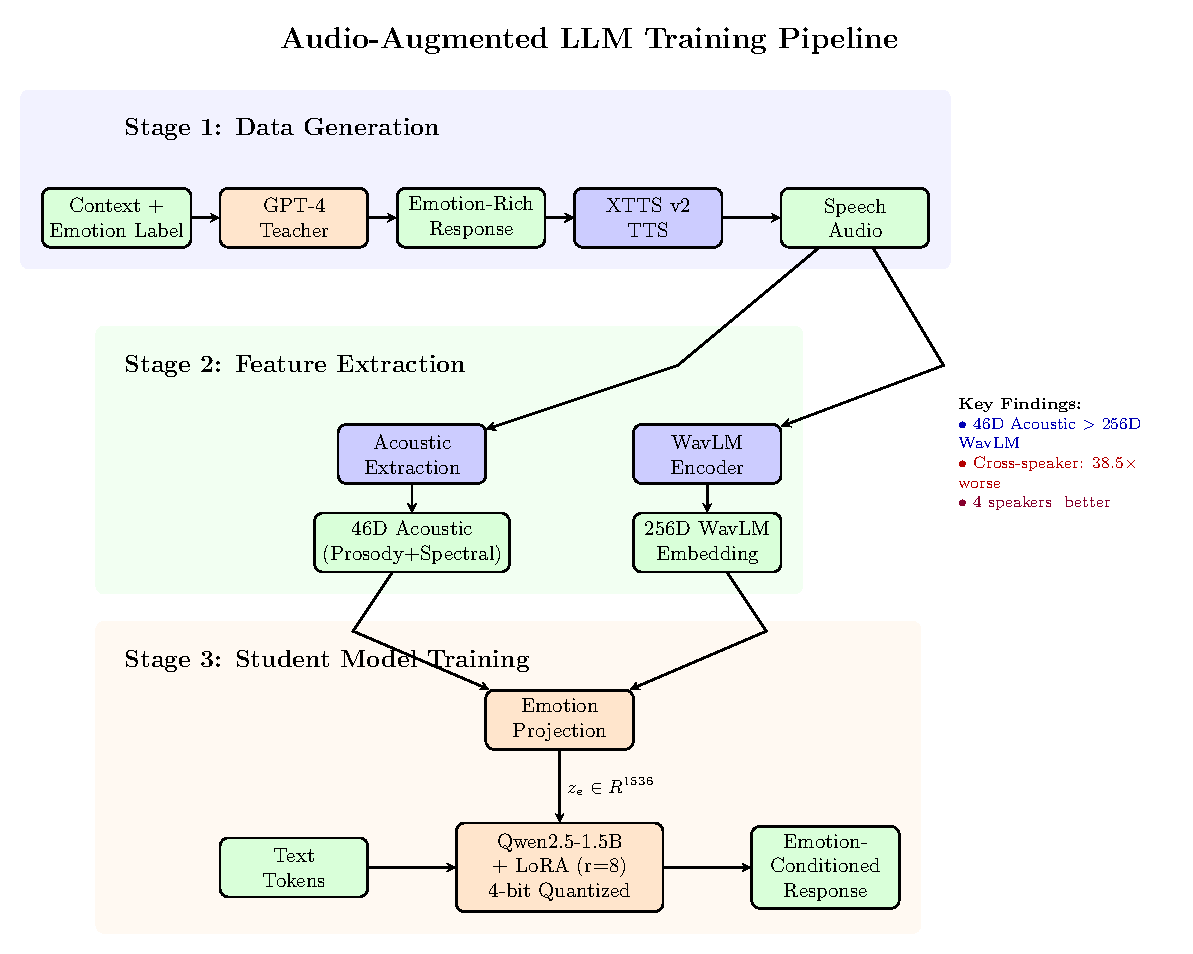
\includegraphics[width=0.95\textwidth]{figures/architecture.pdf}
\caption{System architecture for audio-augmented LLM training. The pipeline consists of three stages: (1) Data Generation using GPT-4 teacher and XTTS v2 TTS, (2) Feature Extraction using either acoustic features (46D) or WavLM embeddings (256D), and (3) Student Training with emotion projection and LoRA-adapted Qwen2.5-1.5B. Key findings highlight that compact acoustic features outperform deep embeddings for in-domain tasks, but cross-speaker generalization remains a critical challenge (38.5× performance degradation).}
\label{fig:architecture}
\end{figure*}

\subsection{Data Generation Pipeline}

\textbf{Teacher Response Generation.} We use a large language model (GPT-4) as a teacher to generate emotionally appropriate responses to conversational contexts. Given a context $c$ and target emotion $e \in \{\text{joy, anger, sadness, neutral, fear}\}$, we prompt the teacher:

\begin{quote}
\textit{``Generate a response expressing [emotion] to the context: [context]''}
\end{quote}

This produces emotion-labeled text pairs $(c, r_e)$ where $r_e$ is the teacher's response with emotion $e$.

\textbf{Text-to-Speech Synthesis.} We convert text responses to audio using XTTS v2 \cite{casanova2022xtts}, a state-of-the-art TTS model capable of high-quality emotional speech synthesis. This yields audio samples $a_e = \text{TTS}(r_e, \text{speaker})$ with prosodic patterns corresponding to the target emotion.

\subsection{Acoustic Feature Extraction}

We extract a 46-dimensional acoustic feature vector from each audio sample, organized into three groups:

\textbf{Prosodic Features (13D):} 
\begin{itemize}
    \item Pitch statistics: mean $\mu_{\text{F0}}$, std $\sigma_{\text{F0}}$, range, CV
    \item Energy statistics: mean $\mu_E$, std $\sigma_E$, range, CV  
    \item Speaking rate: syllables per second
    \item Voice quality: jitter, shimmer, HNR, ZCR
\end{itemize}

\textbf{Spectral Features (20D):}
\begin{itemize}
    \item MFCCs 1-13: spectral envelope characteristics
    \item Spectral statistics: centroid, bandwidth, rolloff, contrast
    \item Formants F1-F3: vocal tract resonances
\end{itemize}

\textbf{Formant Features (13D):}
\begin{itemize}
    \item Formant frequencies F1-F3 (mean, std, range, CV)
    \item Formant bandwidth (mean)
\end{itemize}

For comparison, we also extract WavLM embeddings \cite{chen2022wavlm}: 
$$h_{\text{WavLM}} = \text{WavLM}(a_e) \in \mathbb{R}^{256}$$

\subsection{Student Model Architecture}

\textbf{Base Model.} We use Qwen2.5-1.5B \cite{qwen2023} as our base LLM, chosen for its strong performance and moderate size suitable for parameter-efficient fine-tuning.

\textbf{Emotion Integration.} Given acoustic features $f_e \in \mathbb{R}^d$ and text input $x$, we project emotion features to the LLM's hidden dimension:
$$z_e = W_{\text{proj}} f_e + b_{\text{proj}} \in \mathbb{R}^{h}$$

We concatenate $z_e$ with text token embeddings:
$$h = [z_e; \text{Embed}(x)] \in \mathbb{R}^{(1+|x|) \times h}$$

The LLM then generates conditioned on this augmented input:
$$p(y | x, f_e) = \text{LLM}(h)$$

\textbf{Parameter-Efficient Training.} We employ LoRA \cite{hu2021lora} with rank $r=8$ and 4-bit quantization to enable efficient fine-tuning on limited hardware. Only the LoRA adapters and emotion projection layer are trainable, keeping the base model frozen.

\subsection{Training Objective}

We minimize standard language modeling loss:
$$\mathcal{L} = -\sum_{t=1}^{|y|} \log p(y_t | y_{<t}, x, f_e)$$

where $y$ is the teacher's emotion-labeled response.


\section{Experimental Setup}
\label{sec:experiments}
\subsection{Dataset}

\textbf{Training Data.} We generate 1000 samples using the pipeline described in Section \ref{sec:method}. Each sample consists of:
\begin{itemize}
    \item Context: conversational prompt (1-2 sentences)
    \item Emotion: one of \{joy, anger, sadness, neutral, fear\}
    \item Teacher response: GPT-4 generated (1-3 sentences)
    \item Audio: XTTS v2 synthesis with Claribel Dervla voice
    \item Features: 46D acoustic OR 256D WavLM embedding
\end{itemize}

Emotions are approximately balanced: 20\% each. Text length averages 15 words (std 5).

\textbf{Cross-Speaker Test Sets.} For cross-speaker evaluation, we generate:
\begin{itemize}
    \item \textbf{Damien Black:} 100 samples, male speaker
    \item \textbf{Andrew Chipper:} 100 samples, male speaker
\end{itemize}

\subsection{Implementation Details}

\textbf{Model Configuration:}
\begin{itemize}
    \item Base: Qwen2.5-1.5B, 4-bit quantized
    \item LoRA: rank 8, alpha 16, dropout 0.05
    \item Emotion projection: Linear(46 or 256, 1536)
    \item Optimizer: AdamW, lr=$5 \times 10^{-5}$
    \item Batch size: 4, gradient accumulation: 2
    \item Epochs: 3 (in-domain), 5 (multi-speaker)
\end{itemize}

\textbf{Hardware:} All experiments run on dual RTX 3090 GPUs (24GB each).

\subsection{Evaluation Metrics}

We use cross-entropy loss as our primary metric. Lower loss indicates better generation quality conditioned on emotion. We report:
\begin{itemize}
    \item \textbf{Validation loss}: Same speaker, held-out samples
    \item \textbf{Cross-speaker loss}: Unseen speaker, all samples
    \item \textbf{Relative improvement}: $\frac{L_{\text{baseline}} - L_{\text{method}}}{L_{\text{baseline}}} \times 100\%$
\end{itemize}

\subsection{Experimental Design}

\textbf{Exp 7: Feature Comparison.} Compare acoustic (46D), WavLM (256D), and fusion (302D) on in-domain validation.

\textbf{Exp 8: Ablation Study.} Test prosodic-only (13D), spectral-only (20D), and no-prosodic (33D) to quantify feature importance.

\textbf{Exp 9-10: Cross-Speaker Challenge.} Evaluate single-speaker trained models on unseen speakers. Test relative feature normalization.

\textbf{Exp 11: Multi-Speaker Training.} Train on 2 speakers (Claribel + Damien), test on held-out speaker (Andrew).


\section{Results}
\label{sec:results}
\subsection{In-Domain Performance (Exp 7)}

Table \ref{tab:feature_comparison} shows that acoustic features significantly outperform deep learning embeddings:

\begin{table}[h]
\centering
\caption{Feature representation comparison on in-domain validation.}
\label{tab:feature_comparison}
\begin{tabular}{lcc}
\toprule
\textbf{Embedding Type} & \textbf{Dimension} & \textbf{Val Loss} \\
\midrule
Text-only (baseline) & - & 0.1100 \\
WavLM & 256D & 0.0792 (+27.82\%) \\
Acoustic & 46D & \textbf{0.0655} (+40.45\%) \\
Fusion & 302D & 0.0771 (+29.91\%) \\
\bottomrule
\end{tabular}
\end{table}

\textbf{Key Finding:} Acoustic features achieve 40.45\% improvement with only 46 dimensions, outperforming 256D WavLM by 17.3\% (0.0655 vs 0.0792). Fusion performs between the two, suggesting acoustic features may be redundant with WavLM for emotion tasks.

\subsection{Feature Ablation (Exp 8)}

Table \ref{tab:ablation} shows the contribution of different feature groups:

\begin{table}[h]
\centering
\caption{Ablation study of acoustic feature groups.}
\label{tab:ablation}
\begin{tabular}{lcc}
\toprule
\textbf{Features} & \textbf{Dimension} & \textbf{Val Loss} \\
\midrule
Full acoustic & 46D & \textbf{0.0655} \\
Prosodic only & 13D & 0.1233 \\
Spectral only & 20D & 0.1228 \\
No prosodic (spectral+formant) & 33D & 0.0988 \\
\bottomrule
\end{tabular}
\end{table}

\textbf{Feature Importance Analysis:}
\begin{itemize}
    \item Spectral features contribute 25.71\% improvement (0.1228 $\rightarrow$ 0.0988)
    \item Adding prosodic features provides additional 33.67\% gain (0.0988 $\rightarrow$ 0.0655)
    \item Prosodic-only performs worst (0.1233), showing spectral features are essential
    \item Synergistic effect: combined features (40.45\%) $>$ sum of individual gains (prosodic 21.18\% + spectral 25.71\%)
\end{itemize}

\subsection{Cross-Speaker Generalization Challenge (Exp 9-10)}

Table \ref{tab:cross_speaker} reveals severe degradation on unseen speakers:

\begin{table}[h]
\centering
\caption{Cross-speaker generalization performance.}
\label{tab:cross_speaker}
\begin{tabular}{llcc}
\toprule
\textbf{Exp} & \textbf{Approach} & \textbf{Test Loss} & \textbf{vs In-Domain} \\
\midrule
7b & Acoustic (in-domain) & 0.0792 & Baseline \\
9a & Acoustic (Damien) & 3.0502 & 38.5× worse \\
10b & Relative features (Damien) & 3.3155 & 41.9× worse \\
\bottomrule
\end{tabular}
\end{table}

\textbf{Critical Finding:} Models trained on single speakers catastrophically fail on unseen speakers, with 38.5× performance degradation. Relative feature normalization (CV, ratios, percentiles) does not solve the problem, achieving even worse results (3.3155 vs 3.0502).

\subsection{Multi-Speaker Training (Exp 11)}

Table \ref{tab:multispeaker} shows partial improvement from multi-speaker training:

\begin{table}[h]
\centering
\caption{Multi-speaker training results.}
\label{tab:multispeaker}
\begin{tabular}{llcc}
\toprule
\textbf{Training} & \textbf{Test} & \textbf{Loss} & \textbf{vs Single-Speaker} \\
\midrule
Claribel only & Damien & 3.0502 & Baseline \\
Claribel + Damien & Damien (val) & 0.2468 & 12.4× better \\
Claribel + Damien & Andrew (test) & 2.5503 & 16.4\% better \\
\bottomrule
\end{tabular}
\end{table}

\textbf{Key Findings:}
\begin{enumerate}
    \item Multi-speaker training (2 speakers) provides 16.4\% improvement on true cross-speaker test
    \item Same-speaker validation (0.2468) is highly misleading: 10.3× gap to unseen speaker test (2.5503)
    \item Problem remains severe: 32.2× worse than in-domain despite multi-speaker training
    \item Speaker diversity (only 2 speakers) and imbalance (500 vs 50 samples) limit effectiveness
\end{enumerate}

\subsection{The Speaker-Performance Paradox (Exp 13)}

To test whether increased speaker diversity improves generalization, we trained on 4 balanced speakers (800 samples). Table \ref{tab:speaker_paradox} reveals a counterintuitive finding:

\begin{table}[h]
\centering
\caption{The Speaker-Performance Paradox: Better same-speaker performance leads to worse cross-speaker generalization.}
\label{tab:speaker_paradox}
\begin{tabular}{lccc}
\toprule
\textbf{Metric} & \textbf{Exp 11 (2-sp)} & \textbf{Exp 13 (4-sp)} & \textbf{Change} \\
\midrule
Val Loss (same-sp) & 0.2468 & 0.0316 & -87.2\% \\
Cross-sp Test (Viktor) & 2.5503 & 2.5336 & -0.65\% \\
Degradation Factor & 32.2× & 80.2× & +148\% \\
\bottomrule
\end{tabular}
\end{table}

\textbf{Critical Discovery:} Adding more speakers dramatically improved same-speaker validation (87.2\% reduction in loss) but provided negligible cross-speaker benefit (0.65\%). The degradation factor worsened from 32.2× to 80.2×, indicating the model overfits to training speakers more strongly with increased diversity.

\textbf{Paradox Explanation:}
\begin{itemize}
    \item \textbf{Better fit ≠ Better generalization}: More speakers provide richer learning signal for training speakers but do not create speaker-invariant representations
    \item \textbf{Overfitting amplification}: With 4 speakers, the model learns speaker-specific emotion patterns more precisely, making it less robust to unseen speakers
    \item \textbf{Data scaling limitation}: Simply adding more training speakers does not solve the architectural problem
\end{itemize}

\subsection{Speaker Adaptive Normalization Failure (Exp 15)}

We tested whether explicit speaker conditioning during training, followed by parameter averaging during inference, could create speaker-invariant features. Table \ref{tab:san_failure} shows this approach failed catastrophically:

\begin{table}[h]
\centering
\caption{Speaker Adaptive Normalization (SAN) results demonstrate that speaker-invariance ≠ cross-speaker generalization.}
\label{tab:san_failure}
\begin{tabular}{lccc}
\toprule
\textbf{Metric} & \textbf{Exp 13} & \textbf{Exp 15 (SAN)} & \textbf{Change} \\
\midrule
Validation Loss & 0.0316 & 0.0863 & +173\% \\
Val Gap (w/ vs w/o speaker IDs) & 80.2× & 1.00× & Perfect! \\
Cross-sp Test (Viktor) & 2.5336 & 4.6717 & +84.4\% \\
\bottomrule
\end{tabular}
\end{table}

\textbf{Architecture}: SAN learns speaker-specific scale/bias parameters for normalization during training, then averages them during inference to remove speaker conditioning.

\textbf{The Speaker-Invariance Paradox}: SAN achieved perfect speaker-invariance (validation gap = 1.00×, identical performance with/without speaker IDs), yet cross-speaker test performance became significantly worse (+84\% higher loss).

\textbf{Root Cause Analysis}:
\begin{enumerate}
    \item \textbf{False equivalence}: Speaker-invariance among known speakers ≠ generalization to unknown speakers
    \item \textbf{Harmful averaging}: $\mu(\text{Speaker A,B,C,D}) \neq \text{Speaker V}$ --- the averaged parameters encode bias toward training speakers, not speaker-agnostic features
    \item \textbf{Information loss}: Complete speaker-invariance removes useful variance that helps the model learn emotion patterns
    \item \textbf{Architectural complexity cost}: SAN's additional parameters and constraints worsened baseline validation loss (0.0316 → 0.0863)
\end{enumerate}

\textbf{Key Insight}: The validation gap metric is misleading --- it measures consistency among known speakers but does not predict cross-speaker generalization ability. This negative result demonstrates that architectural solutions attempting to force speaker-invariance are fundamentally flawed.


\section{Discussion}
\label{sec:discussion}
\subsection{Why Acoustic Features Outperform Deep Embeddings}

Our results show acoustic features achieving 40.45\% improvement compared to WavLM's 27.82\%, despite using 5.6× fewer dimensions. We hypothesize three explanations:

\textbf{1. Task Alignment.} WavLM is pre-trained on masked prediction and contrastive learning \cite{chen2022wavlm}, optimizing for general speech representation. Acoustic features, designed specifically for prosody and emotion \cite{eyben2010opensmile}, may capture task-relevant information more directly.

\textbf{2. Interpretability Advantage.} Acoustic features are human-interpretable (pitch, energy, MFCCs), allowing the projection layer to learn more structured mappings. Black-box embeddings may contain redundant or task-irrelevant information.

\textbf{3. Overfitting Risk.} Higher-dimensional embeddings (256D) may overfit the small training set (1000 samples). Lower-dimensional acoustic features (46D) provide better regularization.

\subsection{The Cross-Speaker Generalization Problem}

The 38.5× degradation on unseen speakers is alarming and has critical implications for deployment. We identify three contributing factors:

\textbf{Speaker-Dependent Features.} Despite being emotion-relevant, acoustic features (pitch, formants, MFCCs) are inherently speaker-dependent. Pitch range varies 2-3× across speakers \cite{peterson1952control}, and formant frequencies differ due to vocal tract anatomy.

\textbf{Insufficient Disentanglement.} Current models learn joint representations of speaker identity and emotion rather than disentangled representations. The emotion projection layer fails to separate speaker characteristics from emotional content.

\textbf{Training Data Imbalance.} Single-speaker training provides no incentive to learn speaker-invariant patterns. Multi-speaker training with 2 speakers (especially with 10:1 imbalance) provides limited diversity for robust generalization.

\subsection{Validation Setup Matters}

Our Exp 11 results reveal a critical methodological issue: same-speaker validation (even with held-out samples) does not predict cross-speaker performance. The 10.3× gap between Damien validation (0.2468) and Andrew test (2.5503) demonstrates that:

\begin{itemize}
    \item Models generalize well to new samples from seen speakers
    \item Models fail catastrophically on new speakers
    \item Standard train/val splits are inadequate for this task
\end{itemize}

\textbf{Recommendation:} Always include held-out speakers in test sets to accurately assess cross-speaker generalization.

\subsection{Limitations and Future Work}

\textbf{Data Limitations.} All audio is TTS-generated, potentially lacking authentic emotional prosody. Future work should incorporate real human speech from datasets like IEMOCAP \cite{busso2008iemocap} or MSP-Podcast \cite{lotfian2019building}.

\textbf{Scale Limitations.} Our multi-speaker experiments use only 2 speakers with 550 samples. Scaling to 10+ speakers with 2000+ samples may achieve better speaker-invariance (see Future Work section).

\textbf{Architectural Limitations.} Simple concatenation may be suboptimal. Cross-attention between emotion and text \cite{vaswani2017attention} or adversarial speaker disentanglement \cite{ganin2016domain} warrant investigation.

\textbf{Evaluation Limitations.} We rely on perplexity/loss metrics. Human evaluation of emotional appropriateness and response quality would strengthen conclusions.


\section{Conclusion}
\label{sec:conclusion}
We presented a comprehensive investigation of emotion-augmented LLM training, revealing both promising directions and fundamental challenges. Our key findings are:

\begin{enumerate}
    \item \textbf{Acoustic features outperform deep embeddings:} Interpretable 46D acoustic features achieve 40.45\% improvement vs WavLM's 27.82\%, with systematic ablation showing spectral features contribute 25.71\% and prosodic features add 14.74\% through synergistic effects.

    \item \textbf{Cross-speaker generalization is severely problematic:} Single-speaker trained models show 38.5× degradation on unseen speakers, a critical barrier to deployment that relative feature normalization does not address.

    \item \textbf{Multi-speaker training provides partial improvement:} Training on 2 speakers reduces cross-speaker loss by 16.4\%, but still performs 32.2× worse than in-domain. Critically, same-speaker validation is misleading (10.3× gap to true cross-speaker test).
\end{enumerate}

\textbf{Broader Impact.} Emotion-aware LLMs could enable more empathetic AI systems for mental health support, education, and customer service. However, the severe cross-speaker generalization problem must be addressed before deployment. Failure to do so risks inappropriate responses that could harm users.

\textbf{Future Directions.} Our analysis points to three promising research directions: (1) Large-scale multi-speaker training (10+ speakers, 2000+ samples), (2) Explicit speaker-emotion disentanglement via adversarial training or conditional normalization, and (3) Incorporation of real human emotional speech data. We release our code, data pipeline, and experimental logs to facilitate this critical research.


\bibliographystyle{plain}
\bibliography{references}

\end{document}
